\documentclass{article}
\usepackage{amsmath}
\usepackage{amssymb}
\usepackage{graphicx}
\usepackage{hyperref}
\usepackage[version=4]{mhchem}

\title{Problem 2}
\date{}

\begin{document}
\maketitle

\section*{Problem}
Triangle \(A B C\) is an isosceles triangle. \(B D\) is the altitude to base \(A C\). \(A F\) is the median to \(B C . A F\) meets \(B D\) at \(G\). Find the number of square inches in the area of triangle \(A B G\) if \(B D=234\) and \(A F=195\).\\
\centering
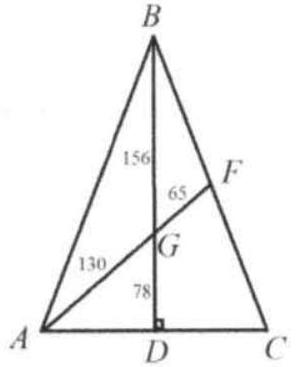
\includegraphics[width=\textwidth]{images/problem_image_1.jpg}

\section*{Solution}
8112.\\
Method 1:\\
\(A F, C E\), and \(B D\) are three medians. They meet at \(G\). Triangle \(A B C\) is divided into six smaller equal areas. \(G D=\frac{1}{3} B D=\frac{1}{3} \times 234=78 . A G=\frac{2}{3} A F=\frac{2}{3} \times 195=130\).\\
Triangle \(A D G\) is a 3-4-5 right triangle \((3 \times 26,4 \times 26,5 \times 26)\) and \(A D=104\).\\
\(S_{\triangle A D G}=\frac{78 \times 104}{2}=4056\)\\
\(S_{\triangle A B G}=2 S_{\triangle M D G}=2 \times 4056=8112\).

Method 2:\\
Note that \(A B C\) is an isosceles triangle, so the altitude is also a median.\\
\(G D=\frac{1}{3} B D=\frac{1}{3} \times 234=78 . A G=\frac{2}{3} A F=\frac{2}{3} \times 195=130\).\\
\(A D=\sqrt{A G^{2}-D G^{2}}=\sqrt{130^{2}-78^{2}}=104\). The area of triangle \(A D G\) is \(S_{\triangle A D G}=\frac{78 \times 104}{2}=4056\).\\
\(\frac{S_{A B G G}}{S_{\triangle A D G}}=\frac{B G}{D G}=2\)\\
\(S_{\triangle A D G}=2 S_{\triangle A D G}=2 \times 4056=8112\).\\
\centering
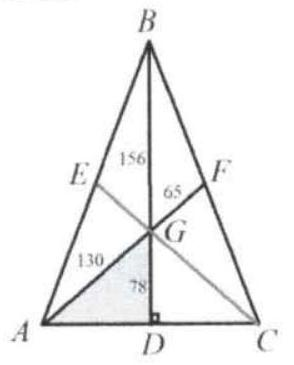
\includegraphics[width=\textwidth]{images/reasoning_image_1.jpg}

\end{document}
